\documentclass[submit]{../harvardml}

\course{CS1810-S25}
\assignment{Homework \#2}
\duedate{February 28, 2025 at 11:59 PM}

\usepackage{float}
\usepackage{../common}
\usepackage[OT1]{fontenc}
\usepackage[colorlinks,citecolor=blue,urlcolor=blue]{hyperref}
\usepackage{graphicx}
\usepackage{subfig}
\usepackage{fullpage}
\usepackage{amsmath}
\usepackage{amssymb}
\usepackage{framed}
\usepackage{color}
\usepackage{soul}
\usepackage{todonotes}
\usepackage{listings}
\usepackage{enumitem}
\usepackage{bm}
\usepackage{bbm}

\usepackage[most]{tcolorbox}
\tcbset{colback=blue!10!white}
\tcbsetforeverylayer{colframe=blue!75!black,breakable}

\newcommand{\B}{\text{B}}
\newcommand{\Beta}{\text{Beta}}

\usepackage[mmddyyyy,hhmmss]{datetime}

\definecolor{verbgray}{gray}{0.9}

\lstnewenvironment{csv}{%
  \lstset{backgroundcolor=\color{verbgray},
  frame=single,
  framerule=0pt,
  basicstyle=\ttfamily,
  columns=fullflexible}}{}
  

%%%%%%%%%%%%%%%%%%%%%%%%%%%%%%%%%%%%%%%%%%%
%% Solution environment
\usepackage{xcolor}
\newenvironment{solution}{
    \vspace{2mm}
    \color{black}\noindent\textbf{Solution}:
}{}
%%%%%%%%%%%%%%%%%%%%%%%%%%%%%%%%%%%%%%%%%%%


\begin{document}

\begin{center}
  {\Large Classification and Bias-Variance Trade-offs}\\
\end{center}

\subsection*{Introduction}

This homework is about classification, bias-variance trade-offs, and
uncertainty quantification.

The datasets that we will be working with relate to astronomical observations and loan applicants
The first dataset, found at \verb|data/planet-obs.csv|,
contains information on whether a planet was observed (as a binary
variable) at given points in time. This will be used in Problem 1. The
second dataset, available at \verb|data/hr.csv|, details different
loan applicants and their measured debt to income ratio and credit score. You will
work with this data in Problem 3.

As a general note, for classification problems we imagine that we have
the input matrix $\boldX \in \reals^{n \times d}$ (or perhaps they
have been mapped to some basis $\bm{\Phi}$, without loss of
generality) with outputs now ``one-hot encoded."  This means that if
there are~$K$ output classes, rather than representing the output
label $y$ as an integer~${1,2,\ldots,K}$, we represent $\boldy$ as a
``one-hot" vector of length~$K$. A ``one-hot" vector is defined as
having every component equal to 0 except for a single component which
has value equal to 1.  For example, if there are $K = 7$ classes and a
particular data point belongs to class 3, then the target vector for
this data point would be~$\boldy = [0,0,1,0,0,0,0]$.  We will define
$C_1$ to be the one-hot vector for the 1st class, $C_2$ for the 2nd
class, etc.  Thus, in the previous example $\boldy = C_3$. If there
are $K$ total classes, then the set of possible labels is $\{C_1
  \ldots C_K \} = \{C_k\}_{k=1}^K$.  Throughout the assignment we will
assume that each label $\boldy \in \{C_k\}_{k=1}^K$ unless otherwise
specified. The most common exception is the case of binary
classification ($K = 2$), in which case labels are the typical
integers $y \in \{0, 1\}$.

\subsection*{Resources and Submission Instructions}

We encourage you to read CS181 Textbook's Chapter 3 for more
information on linear classification, gradient descent, and
classification in the discriminative setting. Read Chapter 2.8 for
more information on the trade-offs between bias and variance.

In problems 1 and 3, you may use \texttt{numpy} or \texttt{scipy}, but
not \texttt{scipy.optimize} or \texttt{sklearn}. Example code is given
in the provided notebook. \textbf{We highly recommend that you use Google Colab for problems 1 and 3 to avoid numerical stability issues.}

Please type your solutions after the corresponding problems using this
\LaTeX\ template, and start each problem on a new page.

Please submit the \textbf{writeup PDF to the Gradescope assignment
  `HW2'}. Remember to assign pages for each question.  Please submit
your \textbf{\LaTeX\ file and code files to the Gradescope assignment
  `HW2 - Supplemental'}. \textbf{You must include your plots in your
  writeup PDF. } The supplemental files will only be checked in
special cases, e.g. honor code issues, etc.


%%%%%%%%%%%%%%%%%%%%%%%%%%%%%%%%%%%%%%%%%%%%%
% Problem 1
%%%%%%%%%%%%%%%%%%%%%%%%%%%%%%%%%%%%%%%%%%%%%

\begin{problem}[Exploring Bias-Variance and Uncertainty]
In this problem, we will explore the bias and variance of a few
different model classes when it comes to logistic regression and
investigate two sources of predictive uncertainty in a synthetic
(made-up) scenario.

We are using a powerful telescope in the northern hemisphere to gather
measurements of some planet of interest. At certain times however, our
telescope is unable to detect the planet due to its positioning around
its star.  The data in \verb|data/planet-obs.csv| records the
observation time in the ``Time" column and whether the planet was
detected in the ``Observed" column (with the value 1 representing that
it was observed).  These observations were taken over a dark, clear
week, which is representative of the region.  Since telescope time is
expensive, we would like to build a model to help us schedule and find
times when we are likely to detect the planet.

\begin{enumerate}
  \item Split the data into 10 mini-datasets of size $N = 30$ (i.e. dataset 1 consists of the first 30 observations, dataset 2 consists of the next 30, etc. This has already been done for you). Consider the three bases $\boldsymbol\phi_1(t) = [1, t]$, $\boldsymbol\phi_2(t) = [1,
          t, t^2]$, and $\boldsymbol\phi_3(t) = [1, t, t^2, t^3, t^4, t^5]$. For each of these bases, fit a logistic regression model using sigmoid($\boldw^\top \boldsymbol\phi(t)$) to each dataset by using gradient descent to
        minimize the negative log-likelihood.  This means you will be
        running gradient descent 10 times for each basis, once for each
        dataset.

        Use the given starting values of $\boldw$ and a learning rate of $\eta=0.001$, take 1,000 update
        steps for each gradient descent run, and make sure to average the
        gradient over the data points at each step. These parameters,
        while not perfect, will ensure your code runs reasonably quickly.

  \item After consulting with a domain expert, we find that the probability of observing the planet is periodic as the planet revolves around its star---we are more likely to observe the planet when it is in front of its star than when it is behind it. In fact, the expert determines that observation follows the generating process $y \sim \text{Bern}(f(t))$, where $f(t) = 0.4 \times \cos(1.1t + 1) + 0.5$ for $t \in [0, 6]$ and $y \in \{0,1\}$. Note that we, the modelers, do not usually see the true data distribution. Knowledge of the true $f(t)$ is only exposed in this problem to allow for verification of the true bias.

        Use the given code to plot the true process versus your learned models. Include your plots in your solution PDF.

        \textbf{In no more than 5 sentences}, explain how bias and variance reflected in the 3 types of curves on the graphs.  How do the fits of the individual and mean prediction functions change?  Keeping in mind that none of the model classes match the true generating process exactly, discuss the extent to which each of the bases approximates the true process.

\end{enumerate}
\end{problem}

\newpage
\begin{framed}
  \noindent\textbf{Problem 1} (cont.)\\
  \begin{enumerate}
    \setcounter{enumi}{2}

    \item If we were to increase the size of each dataset drawn from $N = 30$ to a larger number, how would the bias and variance change for each basis? Why might this be the case? You may experiment with generating your own data that follows the true process and plotting the results, but this is \textbf{not} necessary. \textbf{Your response should not be longer than 5 sentences}.

    \item Consider the test point $t = 0.1$. Using your models trained on basis $\boldsymbol\phi_3$, report the predicted probability of observation of the \textit{first} model (the model trained on the first 30 data points). How can we interpret this probability as a measure of uncertainty? Then, compute the variance of the classification probability over your 10 models at the same point $t = 0.1$. How does this measurement capture another source of uncertainty, and how does this differ from the uncertainty represented by the classification probability? Repeat this process (reporting the first model's classification probability and the variance over the 10 models) for the point $t = 3.2$.

          Compare the uncertainties and their sources at times $t=0.1$ and $t=3.2$.

    \item We now need to make some decisions about when to request time on
          the telescope.  The justifications of your decisions will be sent to
          your funding agency, which will determine whether you will be
          allocated funds to use the telescope for your project. \textbf{In no more than 10 lines}, answer the following questions.
          \begin{itemize}
            \item To identify the ideal time, which model(s) would you use and why?
            \item What time would you request, and why?
            \item Your funding agency suggests using a different telescope in a
                  humid area near the equator. Can you still use your model to
                  determine when the planet is likely to be visible?  Why? Are there
                  adaptations that may be necessary?
            \item You seek out a team that has used the alternative telescope
                  for observing this planet, and they provide you their observation
                  file \verb|data/planet-obs-alternate.csv|.
                  Compare the observations from your telescope to theirs.  What
                  seems to be happening?  What might be an appropriate model for
                  this? Your funding agency asks you to refit your models on these
                  new data.  Do you think this is a reasonable ask, and if so, how
                  will it help you make better decisions about when to request
                  viewing time?  If not, why do you think the additional modeling
                  will not help? You do \emph{not} need to do any modeling for this
                  question!

          \end{itemize}
          In these questions, we are looking for your reasoning; there may be
          more than one valid answer.

  \end{enumerate}
\end{framed}

\newpage

\begin{solution}
    \begin{tcolorbox}
        \textbf{1.} See code.
    \end{tcolorbox}
    \begin{figure}[H]
        \centering
        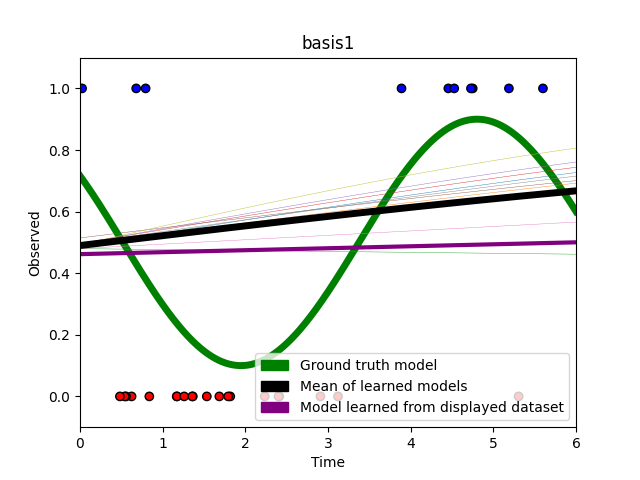
\includegraphics[width=0.6\linewidth]{hw2/imgs/basis1.png}
    \end{figure}
    \begin{figure}[H]
        \centering
        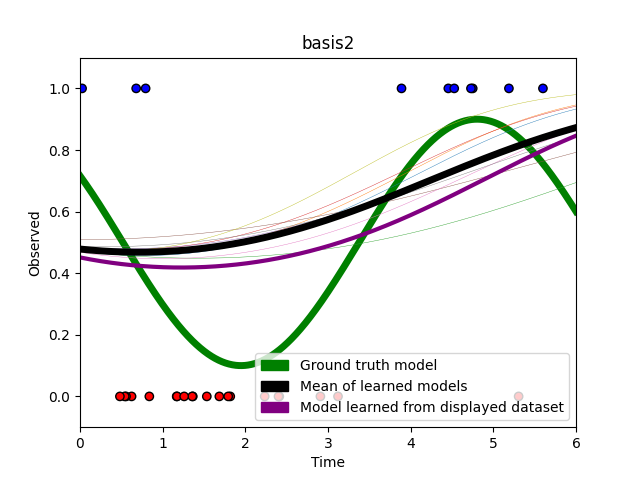
\includegraphics[width=0.6\linewidth]{hw2/imgs/basis2.png}
    \end{figure}
    \begin{figure}[H]
        \centering
        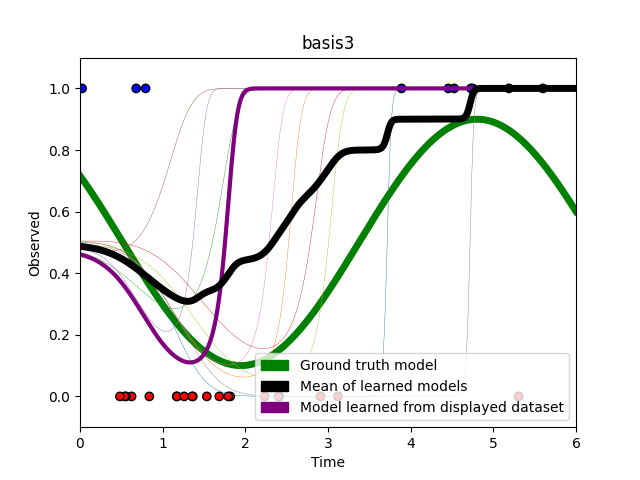
\includegraphics[width=0.6\linewidth]{hw2/imgs/basis3.png}
    \end{figure}
    
    \begin{tcolorbox}
        \textbf{2.} For basis 1, we see that both the mean and individual models are all linear which cannot begin to capture the true sinusoidal shape of the data. Specifically, since the basis is too simple, the resulting models are heavily biased and have low variance, causing the model to underfit to the data. For basis 2, the individual and mean models are very similar and begin to capture some of the periodic trends due to the quadratic transformation, but still suffer from high bias and not enough variance in response to the data. For basis 3, the individual models are heavily influenced by the training data, exhibiting extreme jumps from 0 to 1 which indicate high variance and low bias. This is likely due to basis 3 being too flexible, but it is worth mentioning that the averaged model offers the best fit out of all the transformations to the true data.
    \end{tcolorbox}
    \begin{tcolorbox}
        \textbf{3.} For basis 1, I would expect the bias to remain around the same and variance to slightly lower. For basis 2, I would expect the bias to remain around the same and the variance to decrease. For basis 3, I would expect the bias to remain about the same, but the variance would drastically decrease. This is because increasing the dataset size won't solve a fundamental problem in model flexibility which is measured by bias (ie. including more training samples doesn't change the fact that a simple linear model cannot capture a periodic trend). However, the increased dataset size helps lower variance and overfitting, especially for flexible complex models, since larger samples mean stabler estimates that are less likely to be affected by noise.
    \end{tcolorbox}
    \begin{tcolorbox}
        \textbf{4.} For the probability of observation of the first model, we get the following values
        $$p_{0.1} = 0.499 \quad p_{3.2} = 9.36 \cdot 10^{-6}$$
        For the variance of classification probability over the 10 models, we get
        $$var_{0.1} = 0.0003 \quad var_{3.2} = 0.158$$
        The first type of uncertainty (the probability) is a measure of how certain an individual model is in claiming that there will be an observation at time $t$. That is, it is equivalent to saying "according to model $x$, there is a $p_t$ chance that we observe a star at time $t$. The second type of uncertainty (variance) measures how confident we are that our model itself is accurate. That is, high variance indicates that our models vary greatly in its predicted probability of observation, which tells how much our model is affected by the dataset. Thus, the first metric measures how confident our model is that there will be an observed star at $t$, and the second metric tells us how confident we should be in our model itself.
        \\
        \\
        Comparing the specific uncertainties at time $t = 0.1$ and $t = 3.2$, we see that $p_{0.1} = 0.499 \approx 0.5$. Interpreting this, the model is completely unsure of whether or not there will be an observation at $t = 0.1$, since it determines there is approximately equal chance of either event occurring. However, we are very confident that in our models probability since the variance $var_{0.1} = 0.0003 \approx 0$. Therefore, all 10 of the models give extremely similar probabilities $p_{0.1}$ regardless of their different datasets. On the other hand, $p_{3.2} = 9.36 \cdot 10^{-6} \approx 0$ which indicates that our model is extremely confident that there will be no planets observed at $t = 3.2$. However, $var_{3.2} = 0.158$ which means that we shouldn't be too confident in this probability since it varies relatively largely based on the training dataset. Thus, at $t = 0.1$, the first model is unsure of whether there will be an observation, but we can feel confident in the models prediction. In contrast, at $t = 3.2$, the first model is very confident that there will be no observation, but we shouldn't feel too confident in this since this prediction varies based on the training data.
    \end{tcolorbox}
    \begin{tcolorbox}
        \textbf{5.} To identify the ideal time, I would use the mean learned model using the basis 3 transformation, as it best captures the periodic trends in the data among all the options, albeit imperfectly. The mean model also helps control variance by averaging all the high variance individual models. I would request time $t$ that maximizes my model (averaged model of basis 3) since this is where the predicted observation probability peaks, and we are given no other data. Using a different telescope in a humid area near the equator could pose severable issues, such as obscured observations due to dense clouds or tall trees covering parts of the sky. The new location could introduce confounding periodic trends such as periodic cloud patterns that obscure the observations of the telescope. Thus, adapting the model (such as choosing a new basis) or retraining on new data could be necessary. After visualizing the alternate dataset, the new data has no apparent trends, with the number of observations and non observations staying relatively constant across time. Thus, refitting a temporal regressor would be a waste of resources due to the absence of trends to predict across time.
    \end{tcolorbox}
\end{solution}

%%%%%%%%%%%%%%%%%%%%%%%%%%%%%%%%%%%%%%%%%%%%%
% Problem 2
%%%%%%%%%%%%%%%%%%%%%%%%%%%%%%%%%%%%%%%%%%%%%

\begin{problem}[Maximum likelihood in classification]

Consider now a generative $K$-class model.  We adopt class prior
$p(\boldy = C_k; \bpi) = \pi_k$ for all $k \in \{1, \ldots, K\}$
(where $\pi_k$ is a parameter of the prior).
Let  $p(\boldx|\boldy=C_k)$ denote
the class-conditional density of features $\boldx$ (in this
case for class $C_k$). Consider the data set $D = \{(\boldx_i,
  \boldy_i)\}_{i=1}^n$ where as above $\boldy_i \in \{C_k\}_{k=1}^K$ is
encoded as a one-hot target vector and the data are independent.

\begin{enumerate}
  \item Write out the log-likelihood of the data set, $\ln p(D ; \bpi)$.

  \item Since the prior forms a distribution, it has the constraint that
        $\sum_k\pi_k - 1 = 0$.  Using the hint on
        Lagrange multipliers below, give the
        expression for the maximum-likelihood estimator for the prior
        class-membership probabilities, i.e.
        $\hat \pi_k.$
        Make sure to write out the intermediary equation you need
        to solve to obtain this estimator. Briefly state why your final answer is intuitive.
\end{enumerate}

For the remaining questions, let the
class-conditional probabilities be Gaussian distributions with
the same covariance matrix
$$p(\boldx | \boldy = C_k) = \mathcal{N}(\boldx |  \bmu_k, \bSigma), \text{\ for\ }k \in \{1,\ldots, K\}$$
and different means $\bmu_k$ for each class.

\begin{enumerate}
  \item[3.] Derive the gradient of the log-likelihood with respect to vector $\bmu_k$.
    Write the expression in matrix form as a function of the variables defined
    throughout this exercise. Simplify as much as possible for full credit.
  \item[4.] Derive the maximum-likelihood estimator $\hat{\mu}_k$ for vector $\bmu_k$. Briefly state why your final answer is intuitive.
  \item[5.] Derive the gradient for the log-likelihood with respect to the
    covariance matrix $\bSigma$ (i.e., looking
    to find an MLE for the covariance).
    Since you are differentiating with respect to a
    \emph{matrix}, the resulting expression should be a matrix!
    %
  \item[6.] Derive the maximum likelihood estimator $\hat{\Sigma}$ of the covariance matrix.
\end{enumerate}

\paragraph{Hint: Lagrange Multipliers.} Lagrange Multipliers are a method for
optimizing a function $f$ with respect to an
equality constraint, i.e.
\[\min_{\boldx} f(\boldx)\ \text{s.t.}\ g(\boldx) = 0.\]

This can be turned into an unconstrained problem by introducing a
Lagrange multiplier $\lambda$ and constructing the Lagrangian function,
\[L(\boldx, \lambda) =  f(\boldx) + \lambda g(\boldx).\]

It can be shown that it is a necessary condition that the optimum
is a critical point of this new function. We can find this point by solving two equations:

\[\frac{\partial L(\boldx, \lambda)}{\partial  \boldx} = 0  \ \ \text{and}\  \  \frac{\partial L(\boldx, \lambda)}{\partial \lambda} = 0 \]


\paragraph{Cookbook formulas.} Here are some formulas you might want to consider
using to compute difficult gradients. You can use them  in the homework
without proof. If you are looking to hone your matrix calculus skills, try to
find different ways to prove these formulas yourself (will not be part of the
evaluation of this homework). In general, you can use any formula from the matrix cookbook,
as long as you cite it. We opt for the following common notation:
$\boldX^{-\top} := (\boldX^{\top})^{-1}$
\begin{align*}
   & \frac{\partial \bolda^\top \boldX^{-1} \boldb}{\partial \boldX} = - \boldX^{-\top} \bolda \boldb^\top \boldX^{-\top} \\
   & \frac{\partial \ln | \det (\boldX) |}{\partial \boldX} = \boldX^{-\top}
\end{align*}
\end{problem}

\newpage

\begin{solution}
    \begin{tcolorbox}
        \textbf{1.} First, we have
        $$p(\boldx_i, \boldy_i | \bpi) = p(\boldx_i|\boldy_i) p(\boldy_i | \bpi)$$
        Since $\boldy_i $ is one hot encoded vector where $y_{ik} = 1$ if $y_i = C_k$ and all other $y_{ij} = 0$, then we can write a product of all classes $k$ as
        $$p(\boldx_i, \boldy_i | \bpi) = \prod_{k=1}^K  \left[p(\boldx_i|\boldy_i = C_k) p(\boldy_i = C_k | \bpi)\right] ^{y_{ik}}$$
        Substituting in $p(\boldy_i = C_k | \bpi) = \pi_k$,
        $$p(\boldx_i, \boldy_i | \bpi) = \prod_{k=1}^K  \left[p(\boldx_i|\boldy_i = C_k) \pi_k\right] ^{y_{ik}}$$
        Then, since the data is assumed independent, the likelihood is just the product
        $$p(D; \bpi) = \prod_{i=1}^n \prod_{k=1}^K  \left[p(\boldx_i|\boldy_i = C_k)\pi_k\right] ^{y_{ik}}$$
        Taking the log, we have
        $$\ln p(D; \bpi) = \sum_{i=1}^n \sum_{k=1}^K  y_{ik}(\pi_k + p(\boldx_i|\boldy_i = C_k))$$
        $$\ln p(D; \bpi) = \sum_{i=1}^n \sum_{k=1}^K  y_{ik}\ln(\pi_k) + \sum_{i=1}^n \sum_{k=1}^K  y_{ik}\ln p(\boldx_i|\boldy_i = C_k)$$
    \end{tcolorbox}
    \begin{tcolorbox}
        \textbf{2.} Using the hint on Lagrange multipliers, we construct the Lagrangian function
        $$L(\pi_k, \lambda) = \ln p(D; \bpi) + \lambda (\sum_k\pi_k - 1)$$
        $$L(\pi_k, \lambda) = (\sum_{i=1}^n \sum_{k=1}^K  y_{ik}\ln(\pi_k) + \sum_{i=1}^n \sum_{k=1}^K  y_{ik}\ln p(\boldx_i|\boldy_i = C_k)) + \lambda (\sum_k\pi_k - 1)$$
        Note that since we are differentiating with respect to $\lambda$ and $\pi_k$, the first term in $\ln p(D; \bpi)$ is the only one that matters since the second term is a constant w.r.t $\pi_k$. Therefore
        $$L(\pi_k, \lambda) = \sum_{i=1}^n \sum_{k=1}^K  y_{ik}\ln(\pi_k) + \lambda (\sum_{k=1}^K\pi_k - 1)$$
        Then differentiating and setting to 0 gives us
        $$\frac{\partial L}{\partial \pi_k} = \frac{1}{\pi_k}\sum_{i=1}^n y_{ik} + \lambda = 0$$
        $$\pi_k = -\frac{1}{\lambda}\sum_{i=1}^n y_{ik}$$
        Then w.r.t $\lambda$
        $$\frac{\partial L}{\partial \lambda} =  \sum_{k=1}^K\pi_k - 1 = 0$$
        $$\sum_{k=1}^K\pi_k  = 1$$
        $$\sum_{k=1}^K-\frac{1}{\lambda}\sum_{i=1}^n y_{ik}  = 1$$
        $$\frac{-n}{\lambda} = 1$$
        $$\lambda = -n$$
        Therefore, plugging this back in we have the MLE $\hat\pi_k$ as
        $$\hat\pi_k = \frac{1}{n}\sum_{i=1}^n y_{ik}$$
        Intuitively, this makes sense as a natural MLE for $\pi_k$ would just be the fraction of training points $\boldy_i$ belonging to class $C_k$. This is reflected in the MLE expression since $y_{ik} = 1$ iff $\boldy_i = C_k$, so taking the mean of all $y_{ik}$ gives the proportion as desired.
    \end{tcolorbox}
    \begin{tcolorbox}
        \textbf{3.} If we have 
        $$p(\boldx | \boldy = C_k) = \mathcal{N}(\boldx |  \bmu_k, \bSigma)$$
        Then our log likelihood becomes
        $$\ln p(D; \bpi) = \sum_{i=1}^n \sum_{k=1}^K  y_{ik}\ln(\pi_k) + \sum_{i=1}^n \sum_{k=1}^K  y_{ik}\ln \mathcal{N}(\boldx |  \bmu_k, \bSigma)$$
        $$ =\sum_{i=1}^n \sum_{k=1}^K  y_{ik}\ln(\pi_k) + \sum_{i=1}^n \sum_{k=1}^K  y_{ik} (-\frac{1}{2}(d\ln(2\pi) + \ln(|\bSigma|) + (\boldx_i - \bmu_k)^\top \bSigma^{-1}(\boldx_i - \bmu_k))$$
        $$ = \sum_{i=1}^n \sum_{k=1}^K  y_{ik}\ln(\pi_k) + \sum_{i=1}^n \sum_{k=1}^K -\frac{1}{2} y_{ik} (d\ln(2\pi) + \ln(|\bSigma|)) + \sum_{i=1}^n \sum_{k=1}^K  -\frac{1}{2} y_{ik}(\boldx_i - \bmu_k)^\top \bSigma^{-1}(\boldx_i - \bmu_k)$$
        Using the gaussian PDF. Note that in this complex expresison, the last term is the only relevant term w.r.t $\bmu_k$. All other terms can be treated as constants. In addition, we have $\frac{\partial (x^\top B x)}{\partial x} = 2Bx$ if $B$ is symmetric, which the covariance matrix $\bSigma$ is. Thus using this fact and the chain rule, we get a gradient of
        $$\frac{\partial \ln p(D; \bpi)}{\partial \bmu_k} = 0 + 0 +\sum_{i=1}^n \sum_{k=1}^K -\frac{1}{2}y_{ik}(-2 \bSigma^{-1}(\boldx_i - \bmu_k))$$
        $$ = \bSigma^{-1} \sum_{k=1}^K y_{ik}(\boldx_i - \bmu_k)$$
    \end{tcolorbox}
    \begin{tcolorbox}
        \textbf{4.} To find the MLE $\hat\mu_k$ for $\bmu_k$, we set the gradient we found in part (3) to 0 and solve.
        $$\frac{\partial \ln p(D; \bpi)}{\partial \bmu_k} = \bSigma^{-1} \sum_{k=1}^K y_{ik}(\boldx_i - \bmu_k) = 0$$
        Multiplying by $\bSigma$ and simplifying,
        $$\hat\mu_k = \frac{\sum_{k=1}^K y_{ik}\boldx_i}{\sum_{k=1}^K y_{ik}}$$
        This is intuitive as $\sum_{k=1}^K y_{ik}$ is simply the total number of data points belonging to class $C_k$ and the numerator is simply the sum of all $\boldx_i$ belonging to class $C_k$. Thus, the MLE $\hat\mu_k$ is simply the sample mean of the data $\boldx_i$ that belong to class $C_k$.
    \end{tcolorbox} 
    \begin{tcolorbox}
        \textbf{5.} From part (3), we have the log likelihood:
        $$\ln p(D; \bpi) = $$
        $$\sum_{i=1}^n \sum_{k=1}^K  y_{ik}\ln(\pi_k) + \sum_{i=1}^n \sum_{k=1}^K -\frac{1}{2} y_{ik} (d\ln(2\pi) + \ln(|\bSigma|)) + \sum_{i=1}^n \sum_{k=1}^K  -\frac{1}{2} y_{ik}(\boldx_i - \bmu_k)^\top \bSigma^{-1}(\boldx_i - \bmu_k)$$
        The relevant terms w.r.t $\bSigma$ are
        $$\frac{\partial \ln p(D; \bpi)}{\partial \bSigma} = \frac{\partial}{\partial \bSigma } \biggr(\sum_{i=1}^n \sum_{k=1}^K -\frac{1}{2}y_{ik} \ln(\det|\bSigma|) + \sum_{i=1}^n \sum_{k=1}^K -\frac{1}{2}y_{ik} \ln((\boldx_i - \bmu_k)^\top \bSigma^{-1}(\boldx_i - \bmu_k))\biggr)$$
        We then take the gradient and apply the cookbook formulas to get
        $$\frac{\partial \ln p(D; \bpi)}{\partial \bSigma} = -\frac{n}{2}\bSigma^{-\top} + \frac{1}{2}\sum_{i=1}^n \sum_{k=1}^K y_{ik} \bSigma^{-\top}(\boldx_i - \bmu_k)(\boldx_i - \bmu_k)^\top\bSigma^{-\top}$$
        However, since $\bSigma^{-1}$ is symmetric, then $\bSigma^{-\top} = \bSigma^{-1}$.
        $$\frac{\partial \ln p(D; \bpi)}{\partial \bSigma} = -\frac{n}{2}\bSigma^{-1} + \frac{1}{2} \bSigma^{-1} \biggr(\sum_{i=1}^n \sum_{k=1}^K y_{ik}(\boldx_i - \bmu_k)(\boldx_i - \bmu_k)^\top \biggr) \bSigma^{-1}$$
    \end{tcolorbox}
    \begin{tcolorbox}
        \textbf{6.} Setting the gradient from part (5) to 0 and solving, we get
        $$\frac{\partial \ln p(D; \bpi)}{\partial \bSigma} = -\frac{n}{2}\bSigma^{-1} + \frac{1}{2} \bSigma^{-1} \biggr(\sum_{i=1}^n \sum_{k=1}^K y_{ik}(\boldx_i - \bmu_k)(\boldx_i - \bmu_k)^\top \biggr) \bSigma^{-1} = 0$$
        Multiplying by $\bSigma$ and $2$, we get
        $$ -n\boldI + \biggr(\sum_{i=1}^n \sum_{k=1}^K y_{ik}(\boldx_i - \bmu_k)(\boldx_i - \bmu_k)^\top \biggr) \bSigma^{-1} = 0$$
        $$n\bSigma = \sum_{i=1}^n \sum_{k=1}^K y_{ik}(\boldx_i - \bmu_k)(\boldx_i - \bmu_k)^\top$$
        $$\hat\bSigma = \frac{1}{n}\sum_{i=1}^n \sum_{k=1}^K y_{ik}(\boldx_i - \bmu_k)(\boldx_i - \bmu_k)^\top$$ 
    \end{tcolorbox}
\end{solution}
%%%%%%%%%%%%%%%%%%%%%%%%%%%%%%%%%%%%%%%%%%%%%
% Problem 3
%%%%%%%%%%%%%%%%%%%%%%%%%%%%%%%%%%%%%%%%%%%%%

\begin{problem}[Classifying Loan Applicants]
In this problem, you will code up three different classifiers to classify different types of loan applicants. The file \verb|data/hr.csv| contains data on debt to income ratio measured in tenths of a percent and credit score. The data can be plotted on these two axes:
\begin{center}
  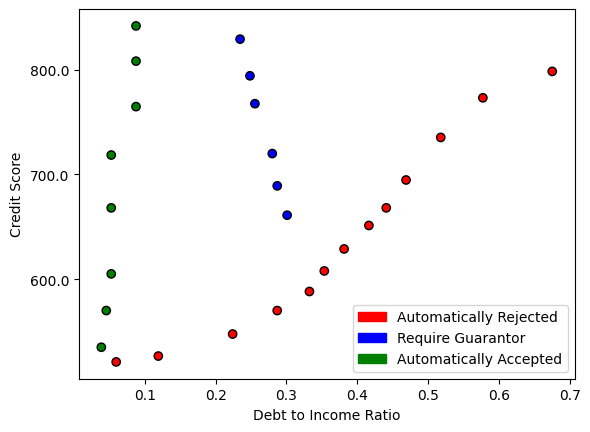
\includegraphics[width=.5\textwidth]{img_input/credit.png}
\end{center}
We've further transformed the raw data on debt to income ratio and credit score so that the default feature vector that you will be working with is defined as such:
\[\bm{x} = \left[\text{debt\_income\_ratio} \cdot \frac{200}{7}-7.5, \frac{\text{credit\_score}-500}{140}-0.5\right]^\top\]

\noindent Please implement the following classifiers in the \verb|SoftmaxRegression| and \verb|KNNClassifier| classes.


\begin{enumerate}[label=\alph*)]

  \item \textbf{A generative classifier with Gaussian class-conditional
          densities with a \textit{shared covariance} matrix} across all classes.
        Feel free to re-use your Problem 2 results.

  \item \textbf{Another generative classifier with Gaussian class-conditional densities , but now
          with a \textit{separate covariance} matrix} learned for each class. (Note:
        The staff implementation can switch between the two Gaussian generative classifiers with just a
        few lines of code.)

  \item \textbf{A multi-class logistic regression classifier} using the softmax activation function. In your implementation of gradient descent, \textbf{make sure to use L2 regularization} with regularization parameter $\lambda = 0.001$. Please also include a bias term, but do not regularize it. Limit the number of iterations of gradient descent to 200,000, and set the learning rate to be $\eta = 0.001$.

  \item \textbf{Another multi-class logistic regression classifier} with the additional feature map:
  $$\phi(\bm x) = [\ln (x_1+10), x_2^2]^\top$$

  \item \textbf{A kNN classifier} in which you classify based on the $k = 1$ and $k = 5$ nearest neighbors and the following distance function: 
  \[\text{dist}(\boldsymbol{x}, \boldsymbol{x}') = (x_1 - x'_1)^2/9 + (x_2 - x'_2)^2\]
        where nearest neighbors are those with the smallest distances from a given point.

        Note 1: When there are more than two labels, no label may have the
        majority of neighbors.  Use the label that has the most votes among
        the neighbors as the choice of label.

        Note 2: The grid of points for which you are making predictions
        should be interpreted as our test space.  Thus, it is not necessary
        to make a test point that happens to be on top of a training point
        ignore itself when selecting neighbors.

\end{enumerate}
\end{problem}

\newpage

\begin{framed}
  \noindent\textbf{Problem 3} (cont.)\\

After implementing the above classifiers, complete the following exercises:
  \begin{enumerate}



      \item Plot the decision boundaries generated by each classifier for the dataset. Include them in your PDF.
            Identify the similarities and differences among the classifiers. What explains the differences---in particular, which aspects or properties of each model dictate the shape of its decision boundary?
    
      \item
    
            Consider a loan applicant with Debt to Income Ratio 0.32 and Credit Score 350. To which class does each classifier assign this applicant? Report the classification probabilities of this applicant for models (c) and (d).
            
            Interpret how each model makes its classification decision. What else should we, the modelers, be aware of when making predictions on a point “far” from our training data? \textbf{Your response should no be longer than 5 sentences.}

    \item
        Can you think of any ethical problem that might arise from using this classifier to make loan decisions? You may approach this from any angle you like. For instance, can you think of someone who might have a low credit score and high debt-to-income ratio that you believe should nonetheless be offered a loan? Are there other variables that should be accounted for to ensure fair decisions? Are credit scores and debt-to-income ratio good bases for loan decisions? More generally, is using a classifier trained on past decisions to determine loan eligibility problematic in any way?
    \end{enumerate}
\end{framed}

\newpage

\begin{solution}
    \begin{figure}[H]
        \centering
        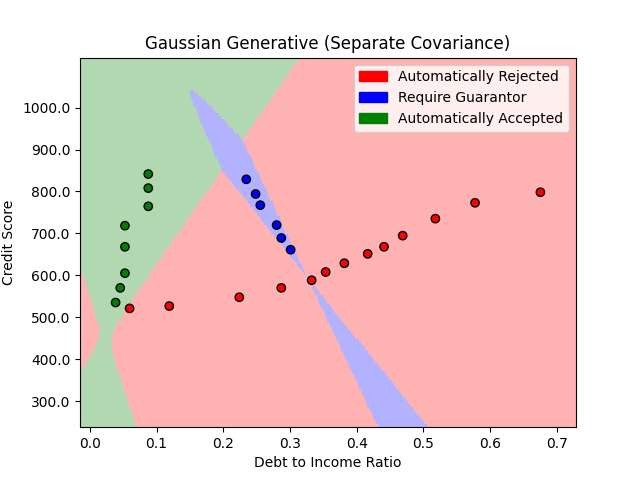
\includegraphics[width=0.7\linewidth]{hw2/imgs/Gaussian Generative (Separate Covariance).png}
    \end{figure}
    \begin{figure}[H]
        \centering
        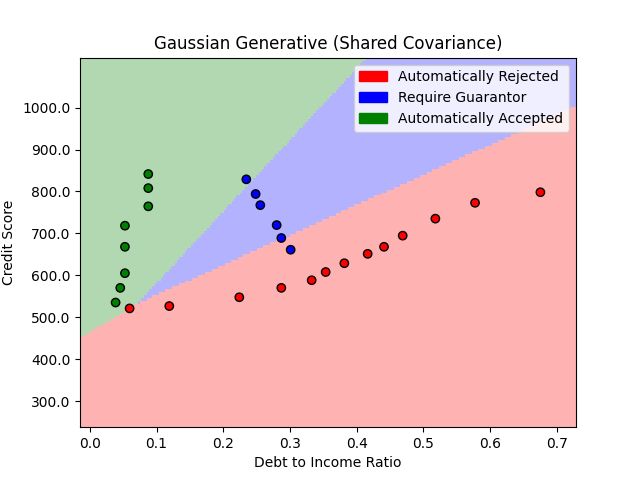
\includegraphics[width=0.7\linewidth]{hw2/imgs/Gaussian Generative (Shared Covariance).png}
    \end{figure}
    \begin{figure}[H]
        \centering
        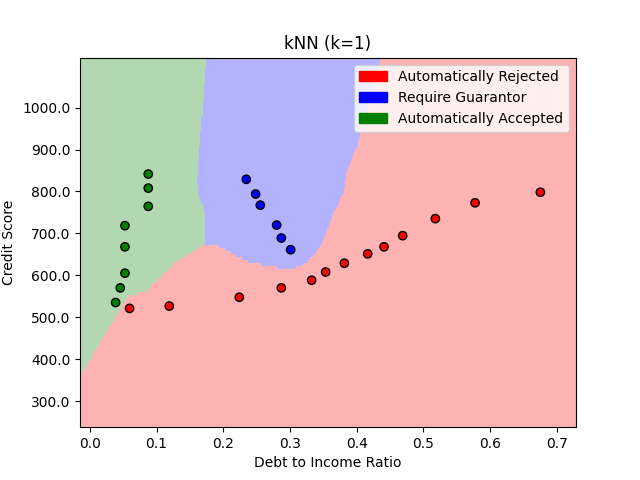
\includegraphics[width=0.7\linewidth]{hw2/imgs/kNN (k=1).png}
    \end{figure}[H]
    \begin{figure}
        \centering
        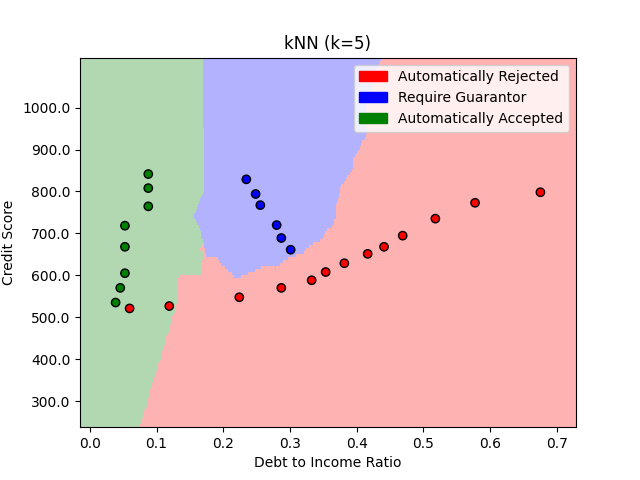
\includegraphics[width=0.7\linewidth]{hw2/imgs/kNN (k=5).png}
    \end{figure}
    \begin{figure}[H]
        \centering
        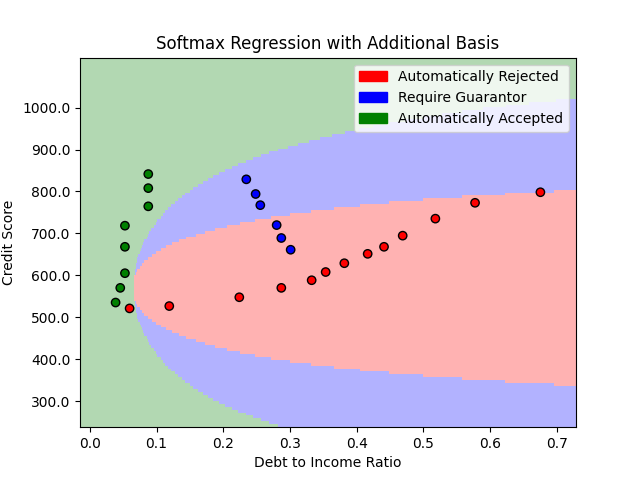
\includegraphics[width=0.7\linewidth]{hw2/imgs/Softmax Regression with Additional Basis.png}
    \end{figure}
    \begin{figure}[H]
        \centering
        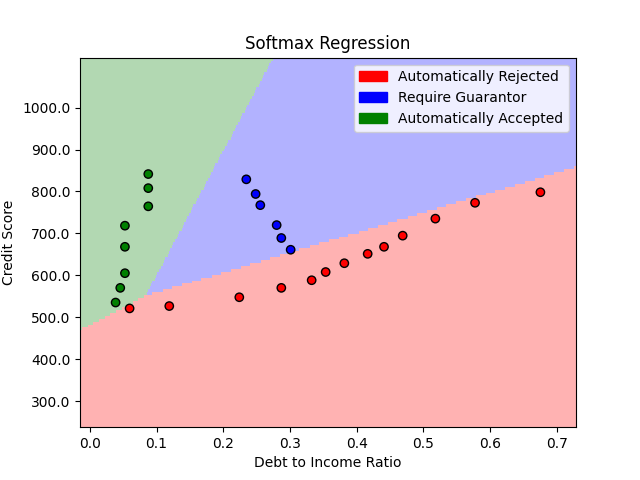
\includegraphics[width=0.7\linewidth]{hw2/imgs/Softmax Regression.png}
    \end{figure}
    
    \begin{tcolorbox}
        \textbf{1.} The KNN models have very similar non linear class boundaries, as is expected. These models make clasification based solely on the nearest neighbors to a point, so it makes sense that the boundaries take form of bulbs around the training data. Notably, for $k = 1$, we see the decision boundary is much more sensitive to individual data points as classification only depends on 1 data point. Meanwhile, for $k=5$, we see the decision boundary better matches our intuitions (classifying people with low debt to income ratio and high credit score as automatically accepts) because of the averaging over multiple neighbors.
        \\
        \\
        The basic softmax regression model and the shared covariance Gaussian model have very similar linear decision boundaries. While the actual mechanism of classification is different-- the softmax attempts to learn weights to draw the decision boundaries while the Gaussian model attempts to learn the underlying distribution of data in each class, they both are very simple and inflexible models. Specifically, the softmax regression model uses a linear basis and thus cannot capture any nonlinear boundaries. The shared covariance Gaussian model assumes that all classes share the same covariance matrix which severely increases the bias of the model (too simple). Thus, although the two models use different classification techniques, the similarity in their boundaries is the result of the over simplicity of their model which fails to capture more complex decision boundaries.
        \\
        \\
        Finally, the Gaussian model with separate covariance matrices and softmax model with an additional basis transform display interesting non linear decision boundaries, although their decision boundaries look very different. The Gaussian model with separate covariance perfectly predicts every data point in the training set yet the actual boundaries make it hard to believe that it will generalize well. Intuitively, this overfitting can be attributed to high model flexibility. By giving each class its own covariance, the number of learnable parameters is greatly increased and the model can learn to perfectly predict every class in the training data. However, this leads to weird and unintuitive boundaries as we can see. 
        \\
        \\
        On the other hand, the softmax regressor with an additional basis also displays non linear behavior, but the decision boundaries are all parabolically shaped. This is a clear reflection of the shape of the additional basis-- although the regressor still tries to draw linear boundaries by learning weights, these linear boundaries are drawn in a new input space which is nonlinear in the original input space.
    \end{tcolorbox}
    \begin{tcolorbox}
        \textbf{2.} Classifiers (a),(b),(c), and (e) assign class 0 (automatically rejected) to this loan applicant, while classifier (d) classifies the loan applicant as class 1 (require guarantor). 
        \\
        \\
        For classifier (c), the probabilities for each class are
        $$p_0 = 3.66297702e-19 \quad p_1 = 9.99986497e-01 \quad p_2 = 1.35033255e-05$$
        Where $p_i$ denotes the probability of being in class $i$. For classifier (d), the probabilities are
        $$p_0 = 2.19082640e-01 \quad p_1 = 7.80866862e-01 \quad p_2 = 5.04984114e-05$$
        The KNN models simply draw boundaries by neighborhoods in the training data set: for a given point in the input space, the model just looks at the nearest other points and assumes classes should be closely clustered. The Gaussian models try to learn the underlying joint distribution behind the data, simply choosing the class that has the highest likelihood of observing a given point. We should be aware that if our training points are far from our training data, then that means that our model predictions are less reliable since they have not seen many of these data points during training and likely have not captured trends farther away from the majority of data. 
    \end{tcolorbox}
    \begin{tcolorbox}
        \textbf{3.} There are many ethical problems for just using classifiers to make loan decisions. For example, as we have seen in the above parts, we cannot guarantee that the models capture the true decision boundaries perfectly. We don't even know if there are "true" decision boundaries in the first place. The real world decision of deciding if someone is eligible for a loan is extraordinarily complex and is tolerant to people with extenuating circumstances. Thus, if the model is trained on data from one inherently biased loan provider, then the model will inherit these biases and treat others with the same prejudice which is unethical. Furthermore, there are many, many more factors that go into credit worthiness other than credit score and income to debt ratio. Therefore, a model like the ones above will be overly simplistic, or put historically marginalized groups at a disadvantage. Moreover, for outlier loan applicants, models will classify them unpredictably which can lead to unethical situations. One example of someone who might be unfairly denied a loan could be someone recently unemployed but who now has a stable job and steady income. While their debt could be high from loans which they needed beforehand, they would likely be able to repay their loan. Overall, using a classifier trained on past decisions is problematic since it amplifies and perpetuates biases, lacks transparency, and harms groups that have hisorically been treated injustly.
    \end{tcolorbox}
\end{solution}

\newpage
%%%%%%%%%%%%%%%%%%%%%%%%%%%%%%%%%%%%%%%%%%%%%
% Name and Calibration
%%%%%%%%%%%%%%%%%%%%%%%%%%%%%%%%%%%%%%%%%%%%%
\newpage

\textbf{Name}: Jaray Liu

\textbf{Collaborators and Resources}: 
\textbf{Collin Fan, Ossimi Ziv}
\end{document}
